\section{Approach}
\label{sec:approach}
{\tool} takes a code fragment as input and searches a code corpus to identify related code fragments. Given a user-selected code fragment, {\tool} first detects it similar methods in the corpus based on syntactic similarity. Then {\tool} traces back to the containing files of these similar methods and identifies other co-occurring methods in these files as candidate related methods. For each candidate related method, we furhter measure its similarity to methods in other files. Then we rank candidate related methods based on the number of similar candidate methods. Figure~\ref{fig:pipeline} describes the pipeline of finding related code fragments in {\tool}. 


\begin{figure}
	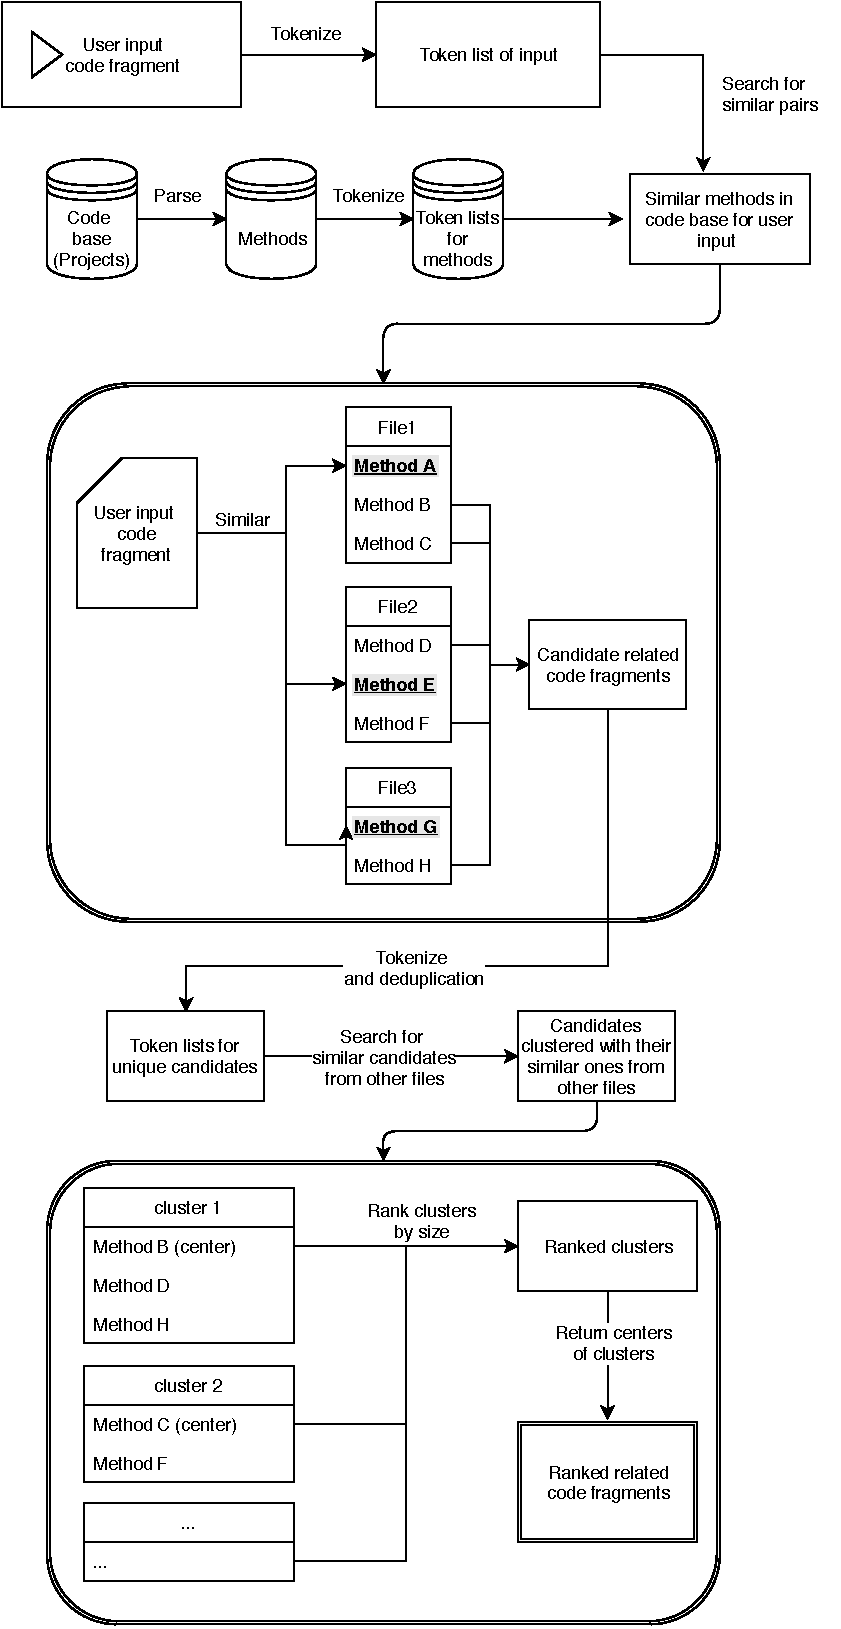
\includegraphics[width=\linewidth]{figures/pipeline.pdf}
	\caption{The pipeline of CodeAid}
	\label{fig:pipeline}
\end{figure}

\subsection{Retrieve similar methods}
\subsubsection{Parse a code corpus}
We focus on method-level code fragments written in Java in this work. We parse all Java source files to abstract syntax trees (ASTs) and traverse the ASTs to extract all defined methods. Note that the approach is not limited to any programming language.

\subsubsection{Tokenization}
Tokenization is the process of transforming source code into a bag of words. Tokenization starts from removing comments, spaces, tabs and other special characters. Then it identifies distinct tokens and count their frequencies. For each method, the result of tokenization is formated as a list of tuples such as {\ttt (token, freq)}, where the first element is a token in the method and the second element refers to the token occurrence in the method.
We tokenize both the input code fragment and all methods in the code corpus, in preparation for the next step of finding similar pairs.

\subsubsection{Search for similar methods}
For the input code fragment, we retrieve its similar counterparts from the code corpus using a token-based clone detection tool called SoucererCC~\cite{sajnani2016sourcerercc}. By evaluating the scalability, execution time, recall and precision of SourcererCC, and comparing it to publicly available and state-of-the-art tools, SourcererCC has been shown to have both high recall and precision, and is able to scale to a large repository using a standard workstation. All of the above make SourcererCC a good candidate for building our code recommendation engine. 
%Given a similarity threshold, SoucererCC takes three steps to detect clones. First, it tokenizes a code snippet to a set of tokens. This tokenization step removes comments, whitespaces, and special characters and also counts the frequency of individual tokens. Second, SoucererCC creates a partial index of each snippet by selecting and indexing a subset of tokens based on heuristics, and builds an inverted index mapping between tokens and code snippets. Finally, SoucererCC iterates through all snippets and finds candidate clones of each snippet by querying the inverted index mapping. After retrieving the candidates, SoucererCC uses another heuristic which exploits ordering of the tokens in a snippet to verify the candidates and locate the clones. 
We use 70\% similarity threshold, because it yields the best precision and recall on multiple clone benchmarks~\cite{sajnani2016sourcerercc}. SourcererCC takes the token lists of the input code fragment and all methods in the code corpus, and returns the similar methods to the input in the code corpus. As shown in Figure \ref{fig:pipeline}, the user input has three similar counterparts in our code corpus, which are {\ttt Method A} in {\ttt File1}, {\ttt Method E} in {\ttt File2}, and {\ttt Method G} in {\ttt File3}.

\subsection{Identify co-occurring code fragments}
Given those similar code fragments identified in the previous step, we trace back to the files that contain these similar counterparts and identify co-occurring methods in the same file as a potentially related code fragment. 

\begin{figure}[h]
		\label{alg: co-occur}
 \removelatexerror
\begin{algorithm}[H]
	\caption{Identify co-ocurring code fragments}
	\KwData{similar methods}
	\KwResult{co-occurring methods}
	initialize $resultList$\;
	\For{$method$ in $similarMethods$}
	{
		$ghFiles$ = traceGitHubFiles(method) \;
		\For{$file$ in $ghFiles$}
		{
			$methodsInFile$ = parse($file$)\;
			\For{$m$ in $methodsInFile$}
			{
				\If {$m$ is not $method$}
				{
					$resultList$.add($m$) \;
				}
			}
		} 
	}
\end{algorithm}
\end{figure}

{\ttt Method A, E, G} are the three similar methods detected by SourcererCC. {\ttt File 1, 2, 3} are the three GitHub files contains these similar methods respectively. 
{\ttt File1} also contains {\ttt Method B, C}, {\ttt File2} contains {\ttt Method D, F}, and {\ttt Method H} is {\ttt File3}. Therefore, {\ttt Method B, C, D, F, H} will be returned as co-occuring methods by Algorithm 1 and they are taken as our candidate for related code fragments.

\subsection{Clustering and Ranking}
\subsubsection{Clustering candidate related code fragments}
We further get the token lists for those candidate related methods identified in the previous step and remove duplicate candidates. in order to detect common co-occurring code fragments, we cluster the remaining unique candidate related methods
based on their token similarity.  Given each candidate related method, we retrieve its token list again and computes its similarity to other candidates which are from different GitHub files. Each candidate will serve as the center of a cluster, we browse among other candidates from other files and add similar candidates to the current cluster.

\begin{figure}[h]
	\label{alg: Clustering candidate related methods}
	\removelatexerror
	\begin{algorithm}[H]
		\caption{Identify co-ocurring code fragments}
		\KwData{$n$ candidate related methods}
		\KwResult{clustered candidate methods}
		initialize $clusters$ = $\{X_1, X_2,..., X_n\}$\;
		\For{$m_i$ in $candidateMethods$}
		{
			$X_i$.add($m_i$) \;
			\For{$m_j$ in $candidateMethods$}
			{
				\If {$m_i$ and $m_j$ do not come from the same file}
				{
					\If {tokenSimilarity($m_i$, $m_j$) $>$ 0.7)}
					{
						$X_i$.add($m_j$);
					}
				}
			} 
		}
	\end{algorithm}
\end{figure}

For the candidate pool above, {\ttt Method B, C, D, F, H}, each candidate will be the center of a cluster. For {\ttt Method B}, we compute token similarity with {\ttt Method D, F, H} and get two similar ones, {\ttt Method D, H}, so we add these two similar methods to the cluster, resulting in cluster size being three. Similarly, we add {\ttt Method F} to the cluster centered by {\ttt Method C} and get a cluster with size two.

\subsubsection{Rank clusters by size}
After getting the candidate clusters, we rank the them by size and return the cluster centers as our final list of related code fragments with ranking. We will recommend {\ttt Method B} first, and then {\ttt Method C}, as our related code fragments.